\documentclass[dvipdfmx,fleqn]{beamer}
\usepackage{amsmath,amsthm,amssymb}
\usepackage{algorithm,algpseudocode}
\graphicspath{{./figure/}{./plot/}}
\makeatletter
\def\input@path{{./figure/}{./table/}}
\makeatother
\usepackage[
sorting=debug,
style=ieee,backend=bibtex,
texencoding=utf8,bibencoding=utf8,
dashed=false,
isbn=false,url=false,doi=false,
sorting=debug
]{biblatex}
\addbibresource{References.bib}
\AtBeginBibliography{}
\setbeamertemplate{bibliography item}[text]
\usetheme{IMELAB}
\usefonttheme[onlymath]{serif}

\usepackage{bxdpx-beamer}
\usepackage{pxjahyper}
\usepackage{verbatim}
%\usepackage[absolute,overlay]{textpos}

\renewcommand{\kanjifamilydefault}{\gtdefault}
\renewcommand{\familydefault}{\sfdefault}

% Theorem
\uselanguage{japanese}
\languagepath{japanese}
\deftranslation[to=japanese]{Theorem}{定理}
\deftranslation[to=japanese]{Lemma}{補題}
\deftranslation[to=japanese]{Example}{例}
\deftranslation[to=japanese]{Examples}{例}
\deftranslation[to=japanese]{Definition}{定義}
\deftranslation[to=japanese]{Definitions}{定義}
\deftranslation[to=japanese]{Problem}{問題}
\deftranslation[to=japanese]{Solution}{解}
\deftranslation[to=japanese]{Fact}{事実}
\deftranslation[to=japanese]{Proof}{証明}
\def\proofname{証明}

% Caption
\renewcommand{\figurename}{図}
\renewcommand{\tablename}{表}

% Beamer Misc.
\usepackage{appendixnumberbeamer}
\setbeamertemplate{navigation symbols}{}
\setbeamertemplate{frametitle continuation}[from second][(続き)]
\setbeamertemplate{section in toc}{\hspace{0.75em}\usebeamercolor[fg]{itemize item}$\blacktriangleright$\hspace{.5em}\usebeamercolor[fg]{normal text}\inserttocsection \\}
\setbeamertemplate{subsection in toc}{\hspace{2em}\usebeamercolor[fg]{itemize item}\inserttocsubsectionnumber\hspace{.5em}\usebeamercolor[fg]{normal text}\inserttocsubsection \\}
\newenvironment{enumalgo}{\begin{enumerate}\scriptsize\setlength\itemsep{0ex}\setlength\leftmargini{0ex}\setlength\leftmarginii{1em}\setlength\leftmarginiii{1em}}{\end{enumerate}}

\title[媒介中心性更新法]{辺操作時の最短経路の更新を利用する \\ 媒介中心性の更新法}
\author[里谷]{里谷 佳紀}
\institute[情数工研]{情報数理工学研究室}
\date[試問]{\alert{試問の名前をかいてね} \\ 2020年2月12日}

\begin{document}

\makeIMELABtitle

\begin{frame}{概要}
  \tableofcontents
\end{frame}

\section{背景・目的}
\begin{frame}[t]{研究背景 -- 媒介中心性}
  \begin{itemize}
  \item \alert{媒介中心性}\footcite{05Freeman1977}:ネットワークのノードの重要度を測る.
  \item[] 例:鉄道網における駅
  \end{itemize}
  \begin{columns}
    \begin{column}{.4\textwidth}
      \begin{equation*}
        B_v=\sum_{s\neq v}\sum_{t\neq v,s}\frac{\sigma_{st}(v)}{\sigma_{st}},
      \end{equation*}
    \end{column}
    \begin{column}{.6\textwidth}
      \begin{itemize}
      \item $\sigma_{st}(v)$:$s$と$t$間の最短経路のうち\\$v$を通るものの数,
      \item $\sigma_{st}$:$s$と$t$間の最短経路の数.
      \end{itemize}
    \end{column}
  \end{columns}
  \medskip
  \begin{itemize}
  \item 媒介中心性の値が高い$\rightarrow$\alert{多くの最短経路が通る}ので重要
  \end{itemize}
  \vspace{-.5em}
  \begin{center}
    %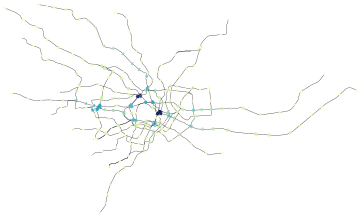
\includegraphics[width=.7\columnwidth]{tokyo-metro-betweenness.pdf}
    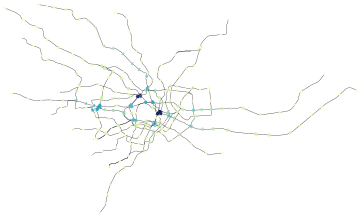
\includegraphics[width=.7\columnwidth]{tokyo-metro-betweenness.png}
  \end{center}
\end{frame}

\begin{frame}{媒介中心性の計算例}
  \begin{columns}
    \begin{column}{.6\textwidth}
      頂点$v$の媒介中心性の値$B_v$は
      \begin{flalign*}
        B_v&=\sum_{s\neq v}\sum_{t\neq s,v}\frac{\sigma_{st}(v)}{\sigma_{st}}\\
        &=\frac{\sigma_{wx}(v)}{\sigma_{wx}}+\frac{\sigma_{wy}(v)}{\sigma_{wy}}
        +\frac{\sigma_{wz}(v)}{\sigma_{wz}}\\
        &+\frac{\sigma_{xy}(v)}{\sigma_{xy}}+\frac{\sigma_{xz}(v)}{\sigma_{xz}}
        +\frac{\sigma_{yz}(v)}{\sigma_{yz}}+\cdots\\
        &=\frac{0}{1}+\frac{0}{1}+\frac{1}{1}+\frac{0}{1}+\frac{2}{2}+\frac{1}{1}\cdots\\
        &=6.
      \end{flalign*}
      同様に,$B_w=B_y=2,\:B_x=B_z=0$.
    \end{column}
    \begin{column}{.39\textwidth}
      \centering
      \def\svgwidth{.9\linewidth}
      \input{graph-bc.pdf_tex}
    \end{column}
  \end{columns}
  \medskip
  計算量:\alert{$\mathcal{O}(|V|^3)$}
\end{frame}

\begin{frame}{Brandesの定理}
  \begin{itemize}
  \item ペア依存度
    $\delta_{s\bullet}(v)=\sum_{t\neq s,v}\sigma_{st}(v)/\sigma_{st}$
  \item 媒介中心性
    $B_v=\sum_{s\neq v}\colorlet{oldcolor}{.}\usebeamercolor[fg]{alerted text}\fbox{$\color{oldcolor}\sum_{t\neq s,v}\sigma_{st}(v)/\sigma_{st}$}\color{oldcolor}=\sum_{s\neq v}\delta_{s\bullet}(v)$
  \item $\delta_{s\bullet}(v)$を高速に計算したい
  \end{itemize}
  \begin{theorem}[Brandes]\rm
    \label{th:implicit-dependency}
    グラフ$G=(V,E)$の異なる頂点$s,v$について,頂点$v$の$s$に対するペア依存度$\delta_{s\bullet}(v)$は次式を満たす.
    \begin{equation*}
      \delta_{s\bullet}(v)=\sum_{(v,w)\in E_s}\frac{\sigma_{sv}}{\sigma_{sw}}(1+\delta_{s\bullet}(w)).
    \end{equation*}
    ただし,$E_s$は$s$から各頂点への最短経路の辺集合である.
  \end{theorem}
  \begin{flushright}
    \alert{次で例を説明}
  \end{flushright}
\end{frame}

\begin{frame}{Brandesのアルゴリズム}
  \begin{columns}
    \begin{column}{.49\textwidth}
      右図において
      \begin{equation*}\small
        \begin{aligned}
          \delta_{s\bullet}(v)&=\frac{\sigma_{sv}}{\sigma_{sw_1}}(1+\delta_{s\bullet}(w_1)) \\
          &+\frac{\sigma_{sv}}{\sigma_{sw_2}}(1+\delta_{s\bullet}(w_2)) \\
          &+\frac{\sigma_{sv}}{\sigma_{sw_3}}(1+\delta_{s\bullet}(w_3))
        \end{aligned}
      \end{equation*}
    \end{column}
    \begin{column}{.49\textwidth}
      \centering
      \def\svgwidth{.9\columnwidth}
      \input{implicit-dependency.pdf_tex}
    \end{column}
  \end{columns}
  \medskip
  \begin{enumerate}
  \item $s$からの最短経路$E_s$を計算
  \item 最短距離の降順に頂点を走査($w$とする)
  \item $(v,w)$が最短経路に含まれるような$v$に対して
  \item[] $\delta_{s\bullet}(v)\gets\delta_{s\bullet}(v)+\colorlet{oldcolor}{.}\usebeamercolor[fg]{alerted text}\fbox{$\color{oldcolor}\sigma_{sv}/\sigma_{sw}(1+\delta_{s\bullet}(w))$}\color{oldcolor}$
  \end{enumerate}
  計算量:\alert{$\mathcal{O}(|V|^2\log |V|+|V||E|)$}
\end{frame}

\begin{frame}{時変ネットワークの媒介中心性}
  \begin{columns}
    \begin{column}{.5\textwidth}
      \begin{itemize}
      \item 現実のネットワークは変化する
      \item[] \alert{時変ネットワーク}
      \item[] 例:フォロー,道路の建設
      \item 時変ネットワークの媒介中心性計算
      \item 影響を受ける部分のみを効率的に計算したい
      \end{itemize}
    \end{column}
    \begin{column}{.5\textwidth}
      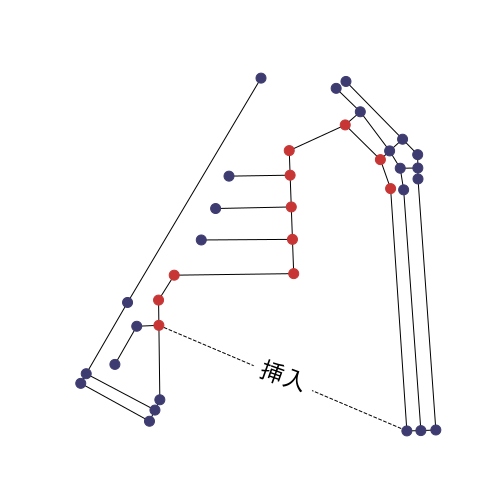
\includegraphics[width=.9\columnwidth]{road-sta.pdf}
    \end{column}
  \end{columns}
\end{frame}

\begin{frame}{関連研究}
  時変ネットワークの媒介中心性更新法
  \begin{itemize}\small
  \item Minimum union cycleを更新\cite{19Lee2012,20Singh2015}
  \item Hypergraph sketch\cite{17Yoshida2014}を更新する\cite{21Hayashi2015},
  \item 近似法を応用\cite{22Bergamini2015a,23Bergamini2015b}
  \item \alert{最短経路と共に媒介中心性を更新}
  \end{itemize}
  \begin{center}
    \scriptsize
    \begin{tabular}{lll}
      \hline
      アルゴリズム & 最短経路更新アルゴリズム & 辺の操作 \\ \hline
      Kasら\cite{25Kas2013} & RamalingamとReps\cite{24Ramalingam1996} & 挿入 \\ \hline
      Nasreら\cite{27Nasre2014a} & Kargerら\cite{26Karger1993} & 挿入 \\ \hline
      Nasreら\cite{29Nasre2014b} & DemetrescuとItaliano\cite{28Demetrescu2003} & 削除 \\ \hline
      Pontecorviら\cite{30Pontecorvi2015} & DemetrescuとItaliano\cite{28Demetrescu2003} & 挿入/削除 \\ \hline
      Bergaminiら\cite{31Bergamini2017} & RamalingamとReps\cite{24Ramalingam1996} & 挿入 \\ \hline
      \alert{本研究} & \alert{RamalingamとReps}\cite{24Ramalingam1996} & \alert{削除} \\ \hline
    \end{tabular}
  \end{center}
  \begin{block}{研究目的}
    \small
    RamalingamとRepsに基づく最短経路更新法を利用する \\
    辺削除時の媒介中心性更新法の提案と評価
  \end{block}
\end{frame}
  
\section{提案アルゴリズム}
\begin{frame}{提案アルゴリズム}
  \alert{TODO}
\end{frame}

\begin{frame}{影響を受ける頂点}
  \alert{TODO}
\end{frame}

\begin{frame}{$\Delta_{s\bullet}(x)$を求めるアルゴリズム}
  \alert{TODO}
\end{frame}

\begin{frame}{最短経路の性質}
  \alert{TODO}
\end{frame}

\begin{frame}{辺削除時の最短経路更新法(Ramalingam and Reps)}
  \alert{TODO}
\end{frame}

\section{数値実験}
\begin{frame}{数値実験}
  \alert{TODO}
\end{frame}

\begin{frame}{Brandes法との性能比較}
  \alert{TODO}
\end{frame}

\begin{frame}{道路ネットワークの媒介中心性の最大値の最小化}
  \alert{TODO}
\end{frame}

\section{まとめ}
\begin{frame}{まとめ}
  \alert{TODO}
\end{frame}

\appendix
\section{参考文献}
\begin{frame}[allowframebreaks]{参考文献}
  \nocite{01Watts1998}
  \nocite{02Barabasi1999}
  \nocite{03Beauchamp1965}
  \nocite{04Bonacich1991}
  \nocite{05Freeman1977}
  \nocite{06Brandes2001}
  \nocite{07Puzis2012}
  \nocite{08Bentert2018}
  \nocite{09Erdos2015}
  \nocite{10Bader2006}
  \nocite{11Tan2009}
  \nocite{12Edmonds2010}
  \nocite{13Bernaschi2016}
  \nocite{14Brandes2007}
  \nocite{15Bader2007}
  \nocite{16Pfeffer2012}
  \nocite{17Yoshida2014}
  \nocite{18Holme2012}
  \nocite{19Lee2012}
  \nocite{20Singh2015}
  \nocite{21Hayashi2015}
  \nocite{22Bergamini2015a}
  \nocite{23Bergamini2015b}
  \nocite{24Ramalingam1996}
  \nocite{25Kas2013}
  \nocite{26Karger1993}
  \nocite{27Nasre2014a}
  \nocite{28Demetrescu2003}
  \nocite{29Nasre2014b}
  \nocite{30Pontecorvi2015}
  \nocite{31Bergamini2017}
  \nocite{32Leskovec2016}
  \nocite{33Rozemberczki2019b}
  \nocite{34OpenStreetMap}
  \printbibliography[title=]
\end{frame}

\end{document}
